\documentclass[journal]{IEEEtran}
\usepackage{amsmath}
\usepackage{amssymb}
\usepackage{graphicx}
\usepackage{fancyhdr}
\usepackage{balance}
\usepackage{enumerate}
\usepackage{epstopdf}
\usepackage{caption}
\usepackage{fixltx2e}
\usepackage{multirow}
\DeclareGraphicsExtensions{.eps}
\ifCLASSINFOpdf
\else
\fi
% correct bad hyphenation here
%\hyphenation{op-tical net-works semi-conduc-tor}

\begin{document}

\title{Hardware-In-the-Loop Testing of Phasor Measurement Unit using Mini-Full Spectrum Simulator}
\author{Rathin Dholakia,~Roll No: 143076001\\M.Tech, Power Electronics and Power Systems,\\ under the guidance of Prof. M. C. Chandorkar, \\ Department of Electrical Engineering, IIT Bombay

\thanks{
}% <-this % stops a space
}
% The paper headers
\markboth{EE 797, M.Tech Project Stage I, 2016}%
{Rathin \MakeLowercase{\textit{et al.}}: MTP Stage-1 Report}
\maketitle
\begin{abstract}
PMU are vital in modern power grid due to advancement in operation and control. Here in this report description of a PMU being developed using OMAP-L137, its testing and verification using a Full Spectrum Simulator (FSS) is discussed. The tests and its standardization reference is taken from smart-grid standard C37.118-2011. While developing the PMU, a custom high speed ADC board is designed, it is interfaced to OMAP using EMIFA - a new interfacing method available in OMAP-L13x processors, is used. This setup will be hooked up to mini-FSS which will provide different test signals. through this experiment we also want to see the usability of FSS in different scenario.
\end{abstract}

\begin{IEEEkeywords}
Wide Area Measurement System(WAMS), Phasor Measurement Unit, IEEE C37.118, Full Spectrum Simulator, OMAP-L137, 
\end{IEEEkeywords}

\IEEEpeerreviewmaketitle
%----------------------------------------------------------------------------------------------------------------------------------------------------
% INTRODUCTION
\section{Introduction}
\IEEEPARstart{D}ay by day power system is becoming more and more complex, which makes it impossible to operate it without automation for higher reliability. Due to wider geographical distribution of the grid, timely detection of faults and taking preventive/corrective countermeasure  has become a complex task, which requires a reliable, fast-acting and absolute technique to deal with the challenge. This is where the Phasor Measurements Unit (PMU) comes in to the picture. Phasor is a complex number which represents both magnitude and angle of an AC quantity. And the synchronized sampling/ measurement of this phasor at a precise reference (time) is called \textbf{synchrophasors} \cite{std:c37}. Using these synchrophasor measurements, different quantities are derived like phase angle, frequency, rate of change of frequency (ROCOF) etc. Frequency is computed as the first derivative of the synchrophasor phase angle and ROCOF is computed as the second derivative of the same phase angle. 

Just like all other engineering devices PMU's reliability, accuracy  and precision are very crucial for its application and hence different kinds of test are done to valididate its performance. Hence just like other measuring devices PMU standards are defined which states minimum performance requirement(s). All device should at least meet the requirement stated by the standards, according their application. 

So, here with this project we are exploring the application of miniaturised Full Spectrum Simulator as a Hardware -in-loop- testing device for PMUs and the implementation of standards on indegenously developed PMU . We will see the feasibility as well as effectivness of the platform and how it can be adjusted to make it suitable for C37.118 compliance testing. This report is largly divided in two parts via three sections 1) C37.118 standard 2) Tests and its explanation and 3) Implemantation. The \textit{compliance} section provides theory background of the topic and basis of tests. Implementation section provides insight about the intended test-setup, hardware detail and the aproach taken. 

\subsection{Background Theory}
Phasor representation of sinusoidal signals is commonly used in AC power system analysis. The sinusoidal waveform defined in Equation (1):

\begin{equation}
x(t) = X_m cos(\omega t + \varphi)
\end{equation}
is commonly represented as the phasor as shown in Equation (2):

\begin{equation}
\textbf{X} = \frac{Xm}{\sqrt{2}}\exp^{j\phi}
or\hspace{2pt} \textbf{X} = X_r+jX_i
\end{equation}

The \textit{synchrophasor} representation of the signal $x(t)$ in Equation (1) is the value X in Equation (2) where $\varphi$ is the instantaneous phase angle relative to a cosine function at the nominal system frequency synchronized to UTC. Before we go into the compliance theory we will go through the basic definations for clarity:\\
\textbf{phasor:} A complex equivalent of a sinusoidal wave quantity such that the complex modulus is the cosine wave amplitude, and the complex angle (in polar form) is the cosine wave phase angle.\\
\textbf{UTC:} Its is the time of day at the earth's prime meridian.\\
\textbf{ROCOF:} It is the measure at which the frequency changes in a give instance of time.\\
\textbf{Rate of change of Frequency Error (RFE):} The measure of error between the theoretical ROCOF and the measured ROCOF for the given instant of time.\\
\textbf{Frame:} A data frame or a frame of data is a set of synchrophasor, frequency, and ROCOF measurements that corresponds to the same time stamp.\\
%----------------------------------------------------------------------------------------------------------------------------------------------------
% INTRODUCTION
\section{C37.118 Standard Compliance}
\IEEEPARstart{E}very PMU should be able to calculate the value of phasor estimate accurately. The estimate will include positive sequence or single phase values, phase difference, freqnency and ROCOF. So it is importnat to keep in mind that the measurements are actually estimates of certain values.

Now, for a given input wave the computation for estimating the desired quantity are given below:
For estimating frequency:
\begin{equation}
f(t) = \frac{1}{2\pi} \dfrac{d\psi(t)}{dt}
\end{equation}
The ROCOF is defined as:
\begin{equation}
ROCOF(t) = \dfrac{df(t)}{dt}
\end{equation}
important thing to note here is that phasors are always computed in relation to the system nominal frequency ($f_0$). Here $\psi(t) = \omega_0 t + \varphi(t)$

\subsection{Measurement Evaluation}
To validate the estimation coming from PMUs they are compared with the theoretical results. As results consists of amplitude and phase difference both they are considered combinedly and this quantity is called \textit{total vector error} (TVE). TVE is an expression of difference between "perfect" sample of a theoretical synchrophasor and the estimate given by the unite at the same instant of time \cite{std:c37}. The value is normalized and expressed in PU of the theoretical phasor:
\begin{equation}
PVE(n) = \sqrt{\frac{ (\hat{X}_r(n) - X_r(n))^2 + (\hat{X}_i(n)-X_i(n))^2} {X_r(n)^2 + X_i(n)^2}}
\end{equation}
Here $ \hat{X}_r (n)$ and $\hat{X}_i(n) $ are the estimated values of the given phasor and $X_r$ and $X_i$ are the theoretical values.
to be complient with standard, PMU shall provide synchrophasor, frequency, and ROCOF measurements that meet the requirements as per the standards at a given time instance \textit{n}. Similarly for freq and ROCOF the validation will be done using following equations:
\begin{eqnarray}
FE == |f_{true}-f_{measured}| = |\Delta f_{true}-\Delta f_{measured}| \\
RFE == |(df/dt)_{true}-(df/dt)_{measured} |
\end{eqnarray}


Apart from the above 3 quantitative parameters other three important parameters to be considered are measurement response time \& delay and reporting delay. \textit{Measurement response time} is the time to transition between two steady-state measurements before and after a step change is applied to the input. \textit{Measurement delay time} is defined as the time interval between the instant that a step change is applied to the input of a PMU and measurement time that the stepped parameter achieves a value that is halfway between the initial and final steady-state values \cite{std:c37}. The reason of measuring time delay is to verify that the time tagging has been compensatated properly or not.  \textit{Latency in reporting} is the time taken between the occurance of even in power system and that being reflacted in the output of the PMU. This parameter largely depends on the class of PMU and the sampling and filtering algorithem used. Which brings us to the classifiction of the PMU, they are divided in two parts:
\begin{enumerate}
\item \textbf{Protection Class (P class):} This PMU is used for protection purposes and hence its response time should be as much less as possible.
\item \textbf{Measurement Class (M class):}  This PMU class emphasies on the accuracy of the reported data and hence timing requirement are not as stringint as P class PMUs.
\end{enumerate} 
%-------------- Hardware Description ------------------ %
\section{Implementation}
Overview of the test setup can be seen in FIGURE, Implementation can be divided in three parts
\begin{enumerate}
\item \textbf{Full Spectrum Simulator (FSS):} Which will have the power system model, through which different test conditions will be given
\item \textbf{PMU:} Which will consist of a ADC interfacing board and OMAP-L 137 EVM
\item \textbf{PC:} It will have a Phasor Data Concentrator (PDC), which receives data from the PMU and record it for future analysis.
\end{enumerate}
During the initial phase of the project intention was to use indegenously PMU developed C-DAC but due to the hardware issues and lack of documentation and support, it was decided that a minimalistic PMU will be developed by ourself.

\subsection{Full Spectrum Simulator:}
As per the requirement of the implementation, miniature-Full spectrum Simulator will be used for this purpose. FSS is a card based, multi CPU - parallel processing hardware.It uses TI's MSP430 DSPs as building block. It was developed by IIT Bombay and CDAC for both, offline \& real-time  simulation purposes in Power Electronics and Power Systems.

\begin{figure}[th]
\centering
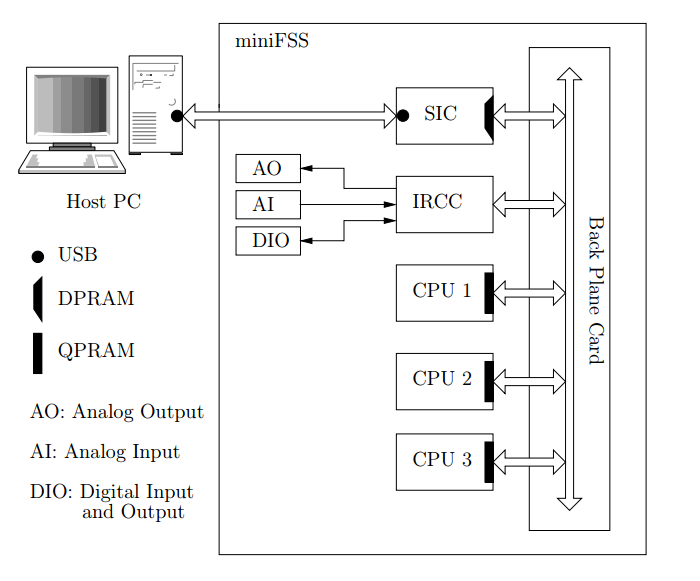
\includegraphics[width=250pt]{fig/fss_arch2.png}
\caption{FSS architecture}
\label{fig:fss_arch}
\end{figure}
As shown in \ref{fig:fss_arch} above it is a card base setup which contains:
\begin{itemize}
\item[-] System Interface Card (SIC)
\item[-] Intra Rack Control Card (IRC Card)
\item[-] Three CPU Cards (CPU 0, CPU 1 and CPU 2), each having 3 digital signal processors on it. So there are total 9 processors allowing for parallel computation.
\item[-] One Analog Output Card (AO Card), having 6 analog output channels (±10 V range).
\item[-]One Analog Input Card (AI Card), having 6 differential analog input channels (±10 V range).
\item[-] One Digital Input/Output Card (DIO Card), having 24 digital inputs and 24 digital outputs (0 - 5 V).
\item[-] One Back Plane PCB.
\end{itemize}


\begin{itemize}
\item \textbf{System Interface Card:} 

It is called SiC, its acts as a communication layer between host PC and the device. Its consists of TUSB chip which connects it to the host PC, a TMS320 to interface SIC with IRC card and a MSP430 to have RS-232 interfacing.
\item \textbf{IRC Card:} IRC is designed as a master control, which eventually control other cards, peripheral communication, timer triggered execution and host pc communication. Further more IRC card handles analog as well as digital input-output also. Apart from that IRC processor also controls the simulation execution using it's timer on the respective CPU card. IRC card has protocal implemented to communicate between CPU cards and SIC so that simulation can be controlled and it's result can be sent to respective peripheral and/or can be downloaded to host PC.

\item \textbf{CPU card:} 

mini-FSS has 3 CPU cards, each having TI's MSP430 DSPs. This card is heart of the FSS. They handle all the mathematical algorithm associated with the simulation. Data flowing from and to the cards are controled by IRC card via \textbf{back plane} PCB.
\end{itemize}

\subsection{PMU}
OMAP-L137 EVM is being used as the platform to design a PMU. OMAP-L137 EVM doesnt have Analog to Digital Converter on board hence a interfacing circuit is developed. While designing the ADC board following criteria were kept considered.
\begin{itemize}
\item Good sampling rate: ~200 Samples/Sec
\item No of channels: 3 + 3 = 6 (3 - $\phi$ voltage and current) 
\item Interfacing type: It should be memory addressable and voltage level compatible  to the EVM.
\item Input type: FSS analog output is differential which can be configured as single. their voltage level is $\pm$10V
\end{itemize}

\begin{figure}[ht]
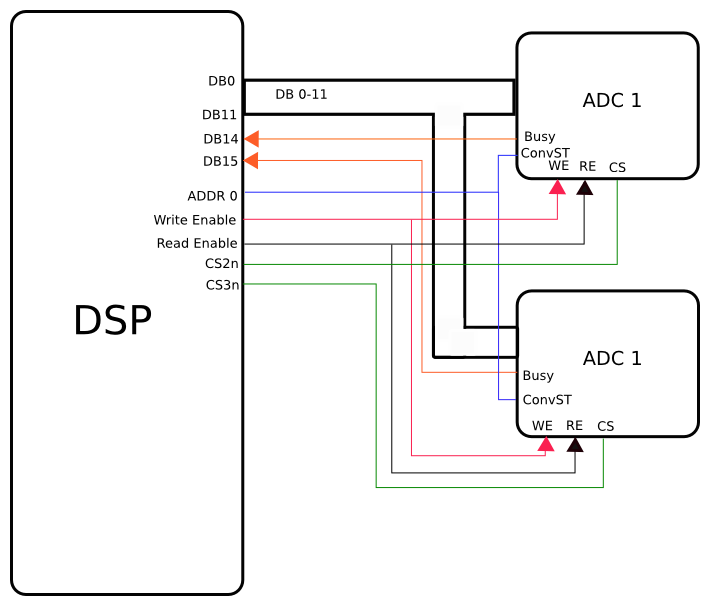
\includegraphics[width=\columnwidth]{fig/ADC_board.png}
\caption{ADC Board block diagram}
\label{fig:adc_board}
\end{figure}
Above Fig:\ref{fig:adc_board} shows the design logic of ADC board. Two AD7864-1 are used as ADC chips due to their high sampling rate of 500 ksps and direct input voltage compatibality range of $\pm$ 10 V. AD7864 is a high speed 4 channel simultaneous sampalling successive approximation ADC with conversion time as low as $1.65 \mu sec$. its conversion sequence can be controlled through hardware as well as software, its default operating voltage is 5v but has a special output voltage shifter for interfacing it with 3.3v processors and controllers. This ADCs are fairly advance hence they have been interfaced with a special asynchronus peripheral interfacing architecture called EMIF-A, which is exclusively available in OMAP-L13x series processors. Extended Memory InterFace (EMIF) has two parts A \& B out of which EMIF-B is having \textit{Enhanced Direct Memory Access} controller (EDMA3) which enables the processor for multi-threaded rapid memory access and hence it is exclusively for highspeed SDRAM interfacing where as interface \textit{A} (EMIF-A) is developed for generic purposes more details are given below:

\subsubsection{EMIF-A}
EMIF-A controller is a 16-bit databus based versetile controller, designed to interact with variety of devices like 
\begin{itemize}
\item Single Data Rate (SDR) RAM
\item Asynchronous devices like NAND \& NOR flash memory and SRAM
\end{itemize}
It contains lot of features to ease and facilitate the usage of asynchronous devices. A functional block diagram is given here in Fig: \ref{fig:EMIFA} 
It is apperent from figure-\ref{fig:EMIFA}, that it has 4 cheap selects and, one read and write and 16 data channels. which makes it very convenient for interfacing multiple peripherals at a time. 
\begin{figure}[ht]
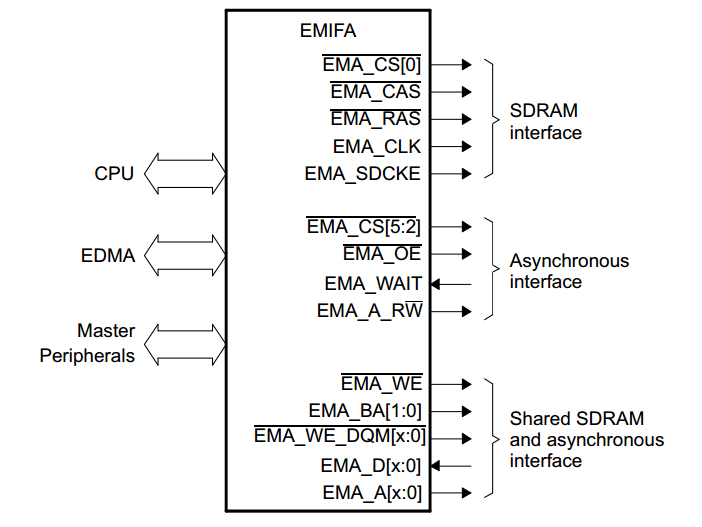
\includegraphics[width=\columnwidth]{fig/EMIFA.png}
\caption{EMIFA Block Diagram}
\label{fig:EMIFA}
\end{figure}

\subsubsection{ADC board Logic}
Due to EMIFA, interfacing of ADC board became quiet convenient rather than using pins in GPIO mode. So the logical flow of the board is as follows:
\begin{itemize}
\item 6 input channels are required hence 2 ICs are used
\item Chip Select (CS), Read, Write, and databits from 0 - 11 are directly available from the EMIFA interface, and they are shared with both the chips.
\item AD7864 has sequence selection which has been configured through hardware, and Clock source has been kept internal. because of this both the pins \texttt{INT/EXT\_CLK} \& \texttt{H/S select}
\item AD7864 has 3 control output \texttt{Busy}, \texttt{FIRSTDATA} and \texttt{EOC}. Out of these only \texttt{busy} is observed via a data line (data bits 16 \& 15). Data is \textbf{and}ed is not read until data line 15 \& 14 are not zero.
\item AD7864 supports two kinds of data reading 1) Reading during the conversion 2)Reading after the conversion. Here we are going to use \textit{Reading After the conversion}, below is the timing diagram of the chip for understanding the proper functioning of the circuit.
\end{itemize}
\begin{figure}[h]
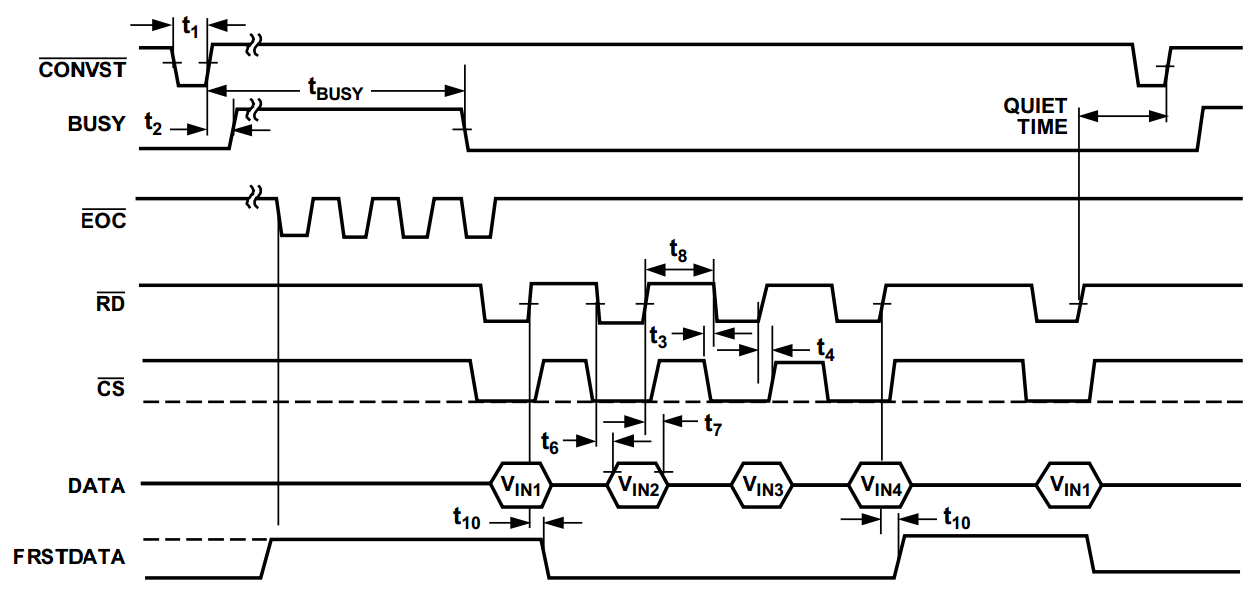
\includegraphics[width = \columnwidth]{fig/adc_time_diag.png}
\caption{ADC Reading After the Convversion timing}
\label{fig:adc_timing}
\end{figure}
Now we will see the operation that takes place when sampling  is to be done:
\begin{itemize}
\item Assert start of conversion (\texttt{CONVST}) is asserted via \texttt{EMA\_CS(4)}
\item Due to this chip will start the conversion processes which will make \texttt{BUSY} high,
\item Status of \texttt{BUSY}  will be checked via \texttt{DB15} \& \texttt{DB14} pins of the EMIFA header, for both the chips untill they are \texttt{low} again.
\item The moment \texttt{BUSY} goes low, \texttt{EMA\_CS[2]} and \texttt{EMA\_A\_RE} are asserted with which AD7864 starts puting data on data lines. this processes of asserting is reapeated for 4 times, for each channel. The same is done using \texttt{EMA\_CS[3]} for getting data from 2nd ADC chip.
\end{itemize}
%\input{algorithm}
%\input{controlactions}
%\input{eigensensitivity}
%\input{casestudies}
%\input{conclusion}
\ifCLASSOPTIONcaptionsoff
  \newpage
\fi
%----------------------------------------------------------------------------------------------------------------------------------------------------
% BIBLIOGRAPHY
\begin{thebibliography}{25}
\bibitem{std:c37}
 C37.118 - IEEE Standard for Synchrophasor Measurements for Power Systems

\bibitem{Book:Padiyar}
Phadke, A.G., Thorp, J.S.,  \textit{Synchronized Phasor Measurements and Their Applications}, Springer US, 2008.

\bibitem{Paper:history}
Phadake A.G., \textit{HISTORY AND APPLICATIONS OF PHASOR MEASUREMENTS}, IEEE, 2006.

\bibitem{Paper:saugata}
Saugata S. Biswas, Jeong Hun Kim, Anurag K Srivastava ``Development of a Smart Grid Test Bed and Applications in PMU and PDC Testing", \textit{IEEE Conference Publications}, 2012.

\bibitem{Paper:ghiga}
R. Ghiga, Q. Wu, K. Martin, W. Z. El-Khatib, L. Cheng and A. H. Nielsen ``Dynamic PMU Compliance Test under C37.118.1aTM-2014", \textit{IEEE PES GM}, PAge 1-5, 2015

\end{thebibliography}
%\input{appendix}

\end{document}